\part{Ethics of analytics}
\frame{\partpage}

\begin{frame}
	\begin{columns}
		\begin{column}{0.48\textwidth}
			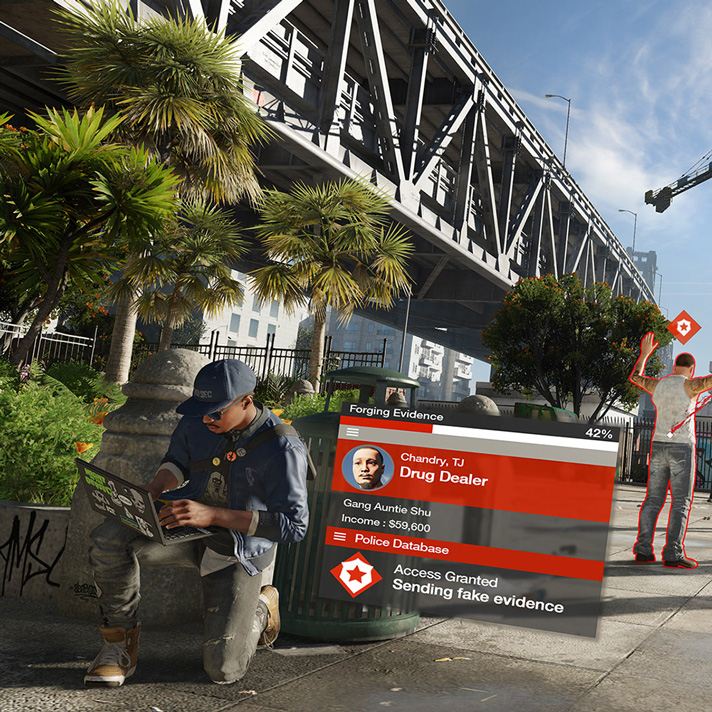
\includegraphics[width=\textwidth]{watch_dogs_2}
		\end{column}
		\pause
		\begin{column}{0.48\textwidth}
			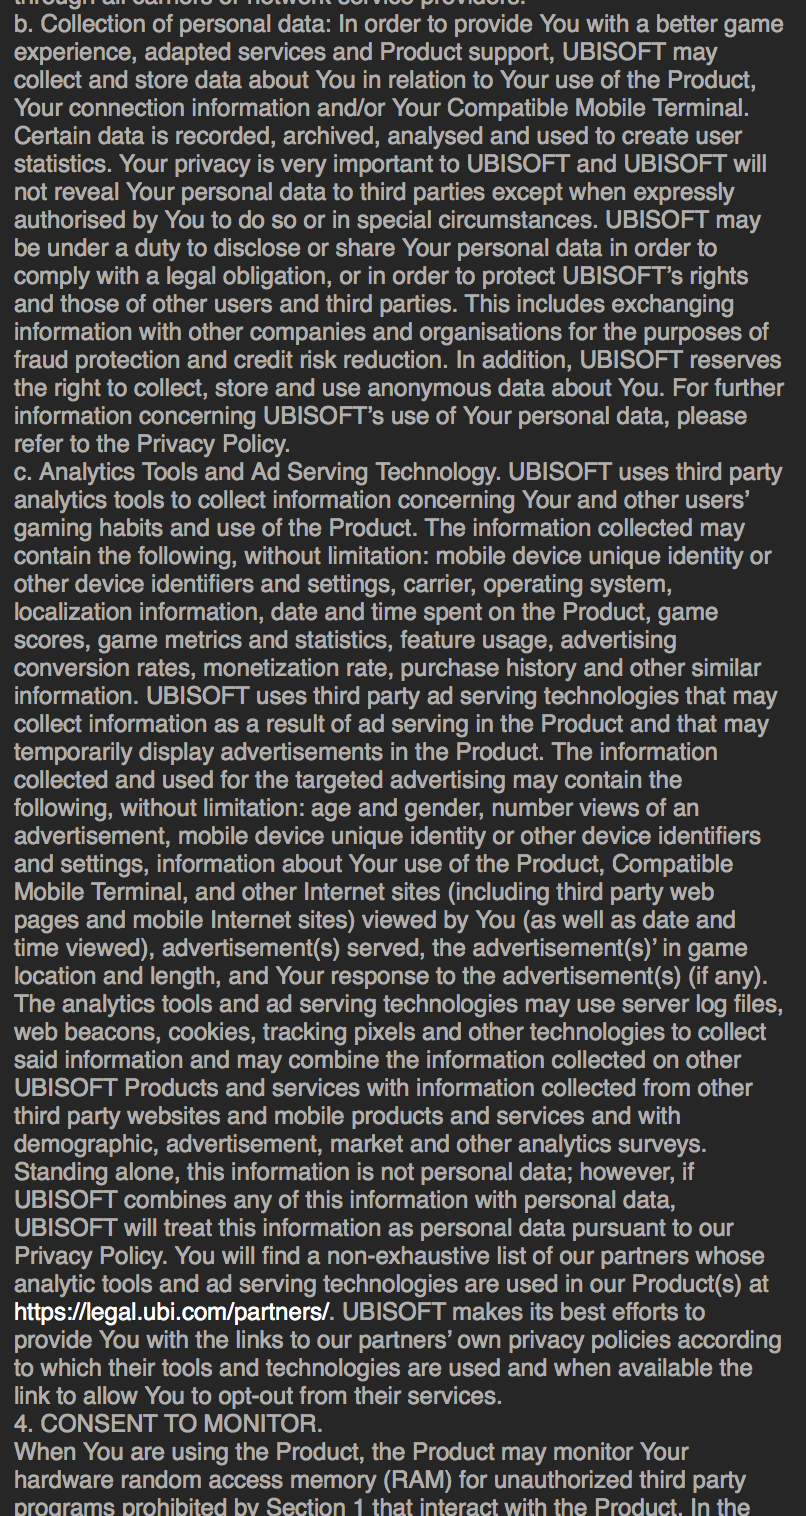
\includegraphics[height=\textheight]{watch_dogs_2_eula}
		\end{column}
	\end{columns}
\end{frame}

\begin{frame}{Ethical considerations}
	\begin{itemize}
		\pause\item Are you breaching your players' \textbf{privacy}?
		\pause\item Is it right to \textbf{experiment} on your players?
		\pause\item Is it right to \textbf{manipulate} your players' behaviour?
		\pause\item Are you deliberately adding \textbf{addictive} qualities to your game?
		\pause\item Is the above justified if it improves the player \textbf{experience}?
		\pause\item What if it improves your \textbf{profits} instead / as well?
	\end{itemize}
\end{frame}

\begin{frame}{The Data Protection Act 1998}
	\begin{itemize}
		\pause\item \textbf{NB: this slide is for education only and does NOT constitute legal advice!}
		\pause\item Covers \textbf{personal data}: any data that can be used to identify a living individual
			\begin{itemize}
				\pause\item Name, phone number, email address, IP address, social media ID, ...
				\pause\item Doesn't cover anonymous data might be OK, depending on how it is anonymised
			\end{itemize}
		\pause\item Covers the \textbf{processing} (including storage) of personal data
		\pause\item The data processor has certain \textbf{responsibilities}
		\pause\item The data subject has certain \textbf{rights}
		\pause\item Not complying with the Data Protection Act can be a \textbf{civil and/or criminal offence}
	\end{itemize}
\end{frame}
